\section{Theory}

\subsection{BLDC Motor Model}
    \label{sec:bldc_theory}

    A brushless DC motor (BLDC) is a synchronous electric motor powered by direct current \cite{PMSM_BOOK}. The torque output of a BLDC motor decreases as its speed increases \cite{Microchip_BLDC}. This relationship is described by the motor's torque-speed curve, shown in Figure \ref{fig:bldc_torque_speed}. The curve is defined by four key parameters: peak torque, maximum speed, rated speed, and rated torque. The rated torque is the maximum continuous torque output, while rated speed is the highest speed at which rated torque can be maintained. Above rated speed, torque output decreases. The motor can briefly exceed rated torque, for example during acceleration, within the limits of the torque-speed curve.

    \begin{figure}[H]
        \centering
        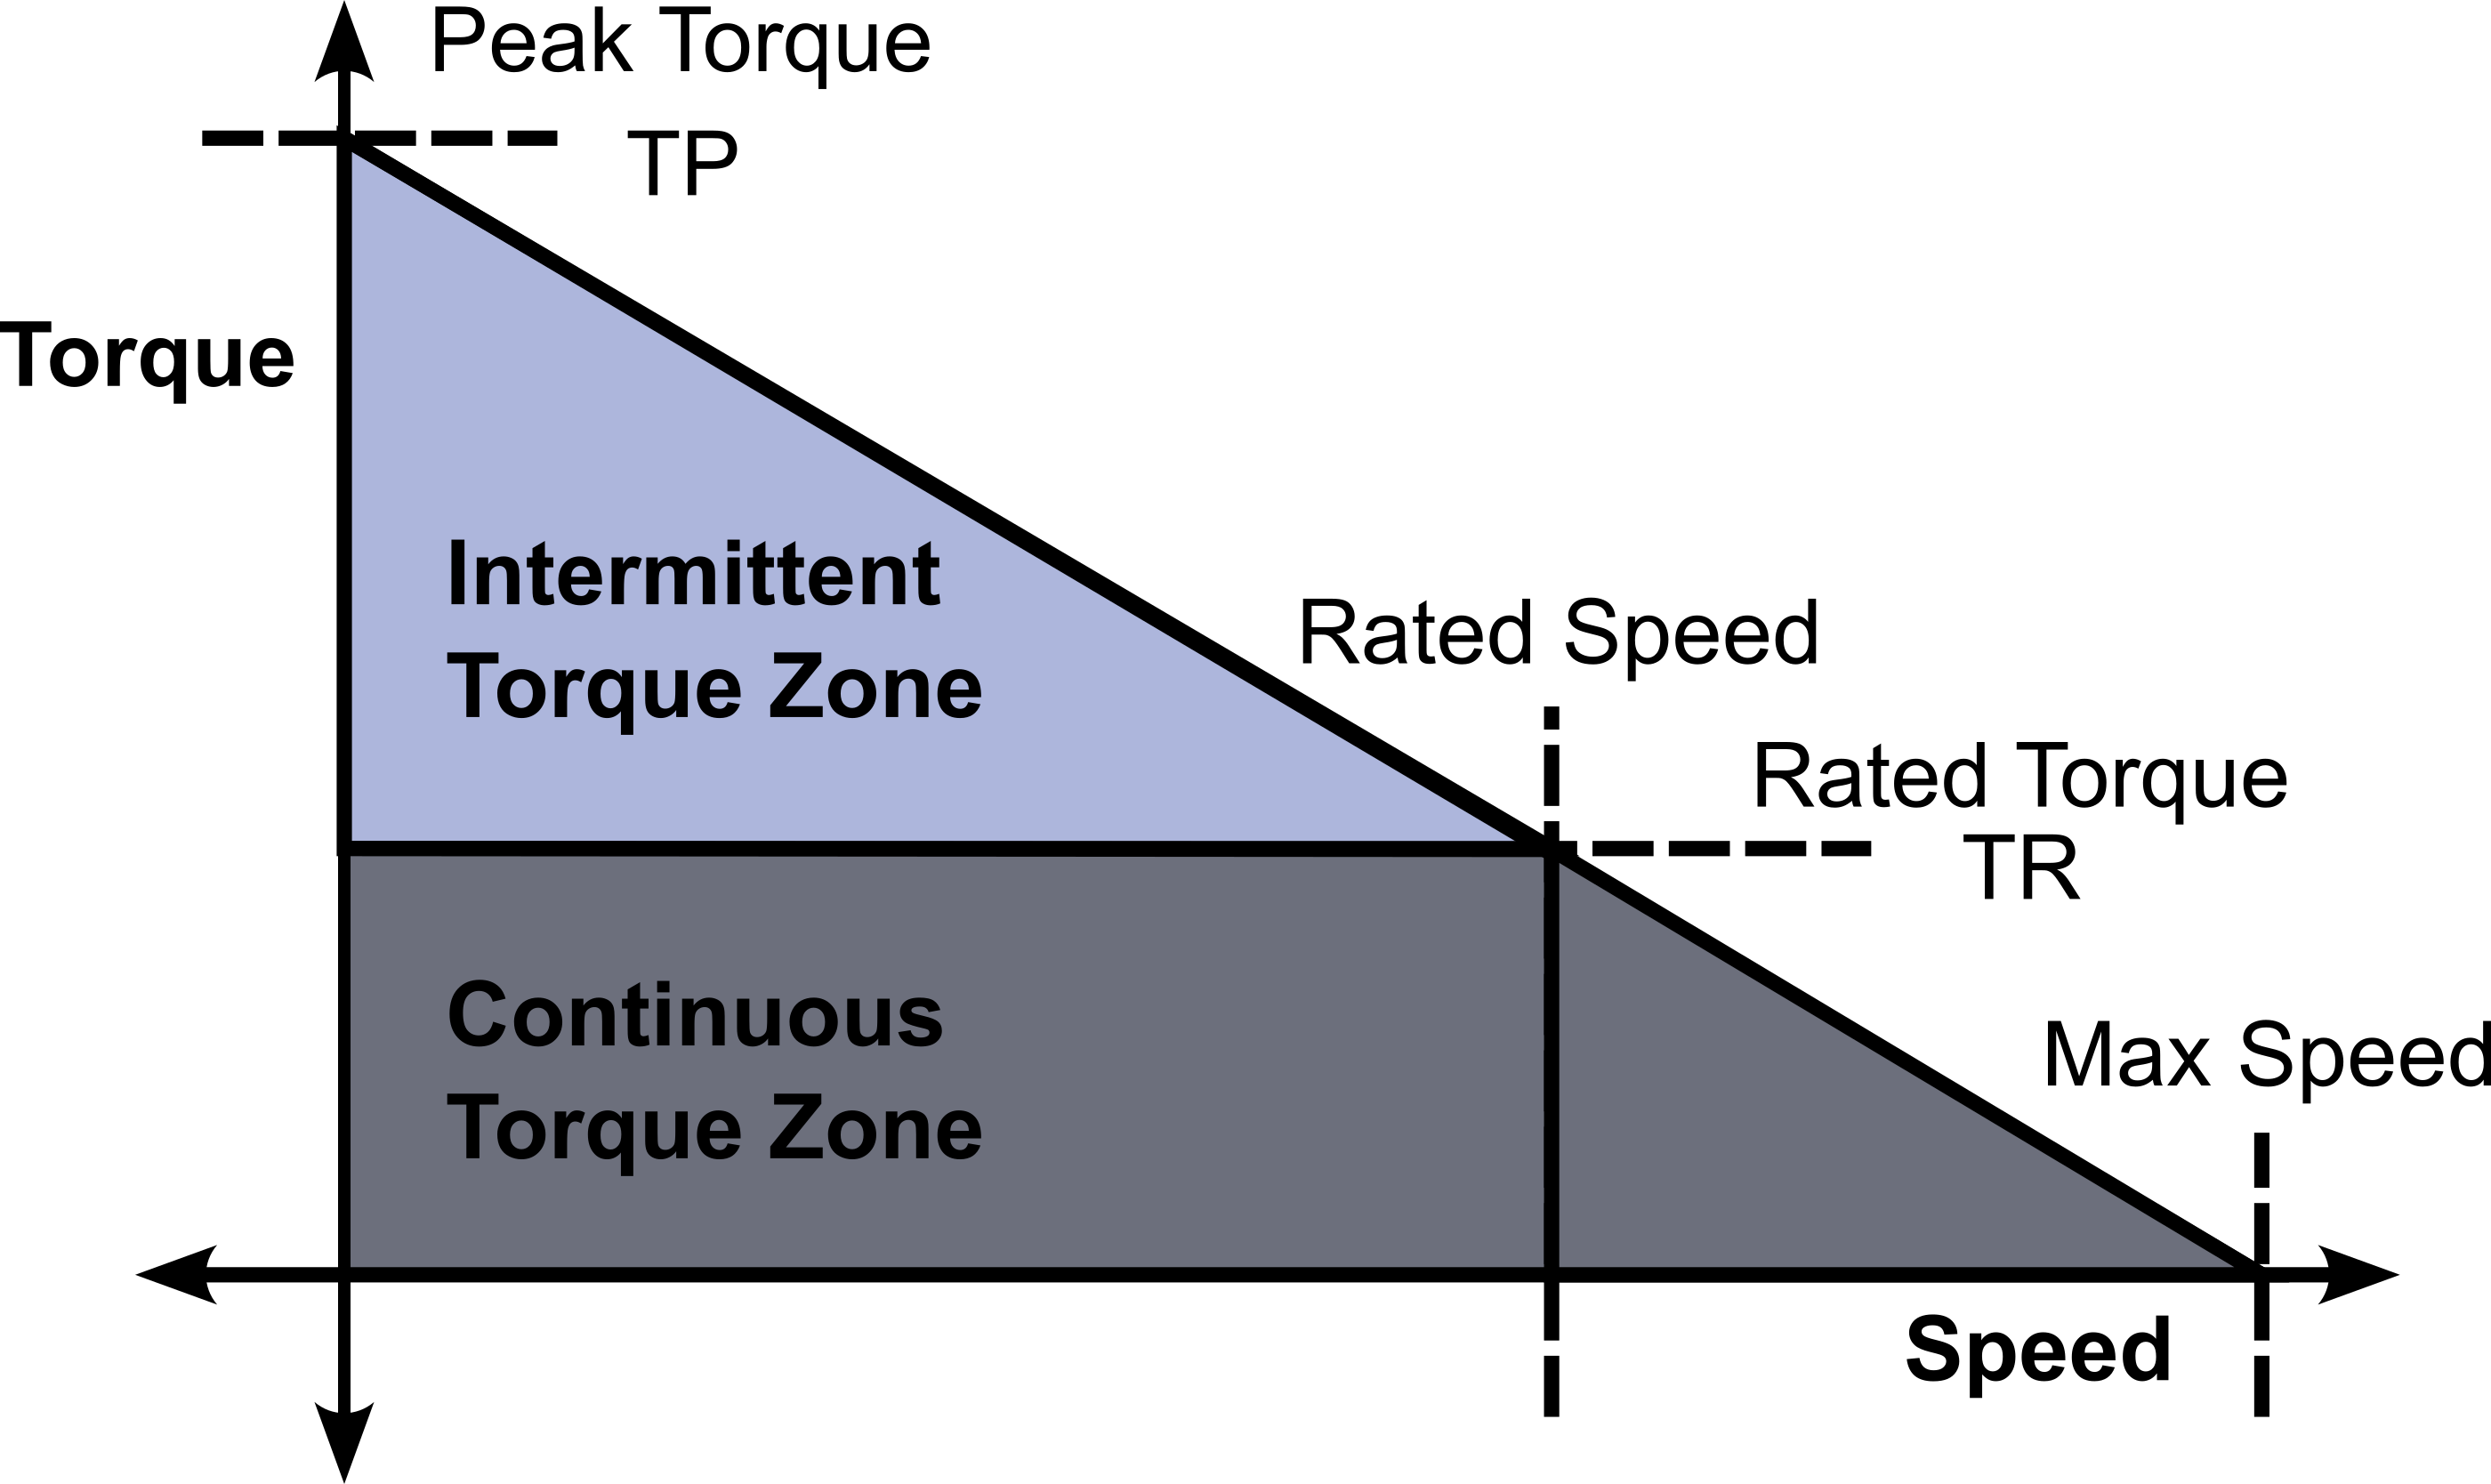
\includegraphics[width=\textwidth]{Images/torque_speed_own.png}
        \caption{Typical torque-speed characteristics of a Brushless DC (BLDC) motor \cite{Microchip_BLDC}. }
        \label{fig:bldc_torque_speed}
    \end{figure}

    When selecting a motor for an application, a 20\% safety margin should be added to the required peak torque, after accounting for friction and other known factors \cite{Microchip_BLDC}.

\subsection{Gear Transmission Friction Model}
\label{sec:gear_transmission_friction_model}

    Electric motors used in robotics often operate at speeds too high and torques too low for direct use. Gear transmissions are used to reduce speed and increase torque.

    In an ideal geared transmission with no power loss, the output torque and velocity are given by equations \ref{eq:gear_torque} and \ref{eq:gear_velocity}, where $N$ is the gear ratio, $\tau_{in}$ and $\tau_{out}$ are input and output torques, and $w_{in}$ and $w_{out}$ are input and output velocities \cite{modern_robotics_book}.

    \begin{equation}
        \label{eq:gear_torque}
        \tau_{out} = N \tau_{in}
    \end{equation}

    \begin{equation}
        \label{eq:gear_velocity}
        w_{out} = \frac{w_{in}}{N}
    \end{equation}

    Real transmissions experience power loss through friction. A common friction model combines viscous friction (proportional to velocity) and Coulomb friction (constant opposing force) \cite{modern_robotics_book}. The total friction torque is the sum of these components, as shown in equation \ref{eq:friction_torque}. Either term may be omitted depending on the application.

    \begin{equation}
        \label{eq:friction_torque}
        \tau_{friction} = b_{viscous}\dot{\theta} + b_{coulomb}\text{sign}(\dot{\theta})  
    \end{equation}

    High gear ratios also increase the apparent rotor inertia. As shown in equation \ref{eq:rotor_kinetic_energy}, apparent inertia increases with the square of the gear ratio \cite{modern_robotics_book}. This can be problematic in robotic applications, particularly during contact, where high apparent inertia leads to stiff impacts \cite{proprioceptive}.

    \begin{equation}
        \label{eq:rotor_kinetic_energy}
        K = \frac{1}{2}{I}_{rotor}(G\dot\theta)^2 = \frac{1}{2}{I}_{rotor}G^2(\dot\theta)^2 = \frac{1}{2}I_{apparent}(\dot\theta)^2
    \end{equation}

\subsection{Spring Modelling}
\label{sec:spring_theory}
Springs store potential energy through elastic deformation. The two main types relevant to this work are linear (extension/compression) springs and torsional springs.

Linear springs develop force proportional to displacement from their free length. For an ideal linear spring, this relationship follows Hooke's Law:
\begin{equation}
    F = -kx
\end{equation}
where $F$ is the spring force, $k$ is the spring constant, and $x$ is displacement from equilibrium. The stored potential energy is:
\begin{equation}
    U = \frac{1}{2}kx^2
\end{equation}

Torsional springs develop torque proportional to angular displacement from their free position:
\begin{equation}
    \tau = -k\theta
\end{equation}
where $\tau$ is the restoring torque, $k$ is the torsional stiffness in Nm/rad, and $\theta$ is the angular displacement. The stored elastic potential energy is:
\begin{equation}
    U = \frac{1}{2}k\theta^2
\end{equation} 

Both spring types are used in mechanical systems for force/torque generation, shock absorption, and energy storage.

\subsection{Kinematics}
    \subsubsection{Robot Kinematics}
    \label{sec:robot_kinematics}
Consider a planar robotic arm with $n$ links, each with length $l_i$ and joint angle $\theta_i$. The end-effector position $\bm{x} = [x, y]^T$ in global coordinates is given by equation \ref{eq:robot_kinematics}, derived from basic trigonometry. Figure \ref{fig:robotic_link_arm} shows the coordinate system and joint angles.

\begin{equation}
    \label{eq:robot_kinematics}
    \bm{x} = \begin{bmatrix}
        x \\
        y
    \end{bmatrix} = \begin{bmatrix}
        \sum_{i=1}^{n} l_i \cos\left(\sum_{j=1}^{i} \theta_j\right) \\
        \sum_{i=1}^{n} l_i \sin\left(\sum_{j=1}^{i} \theta_j\right)
    \end{bmatrix}
\end{equation}

\begin{figure}[H]
    \centering
    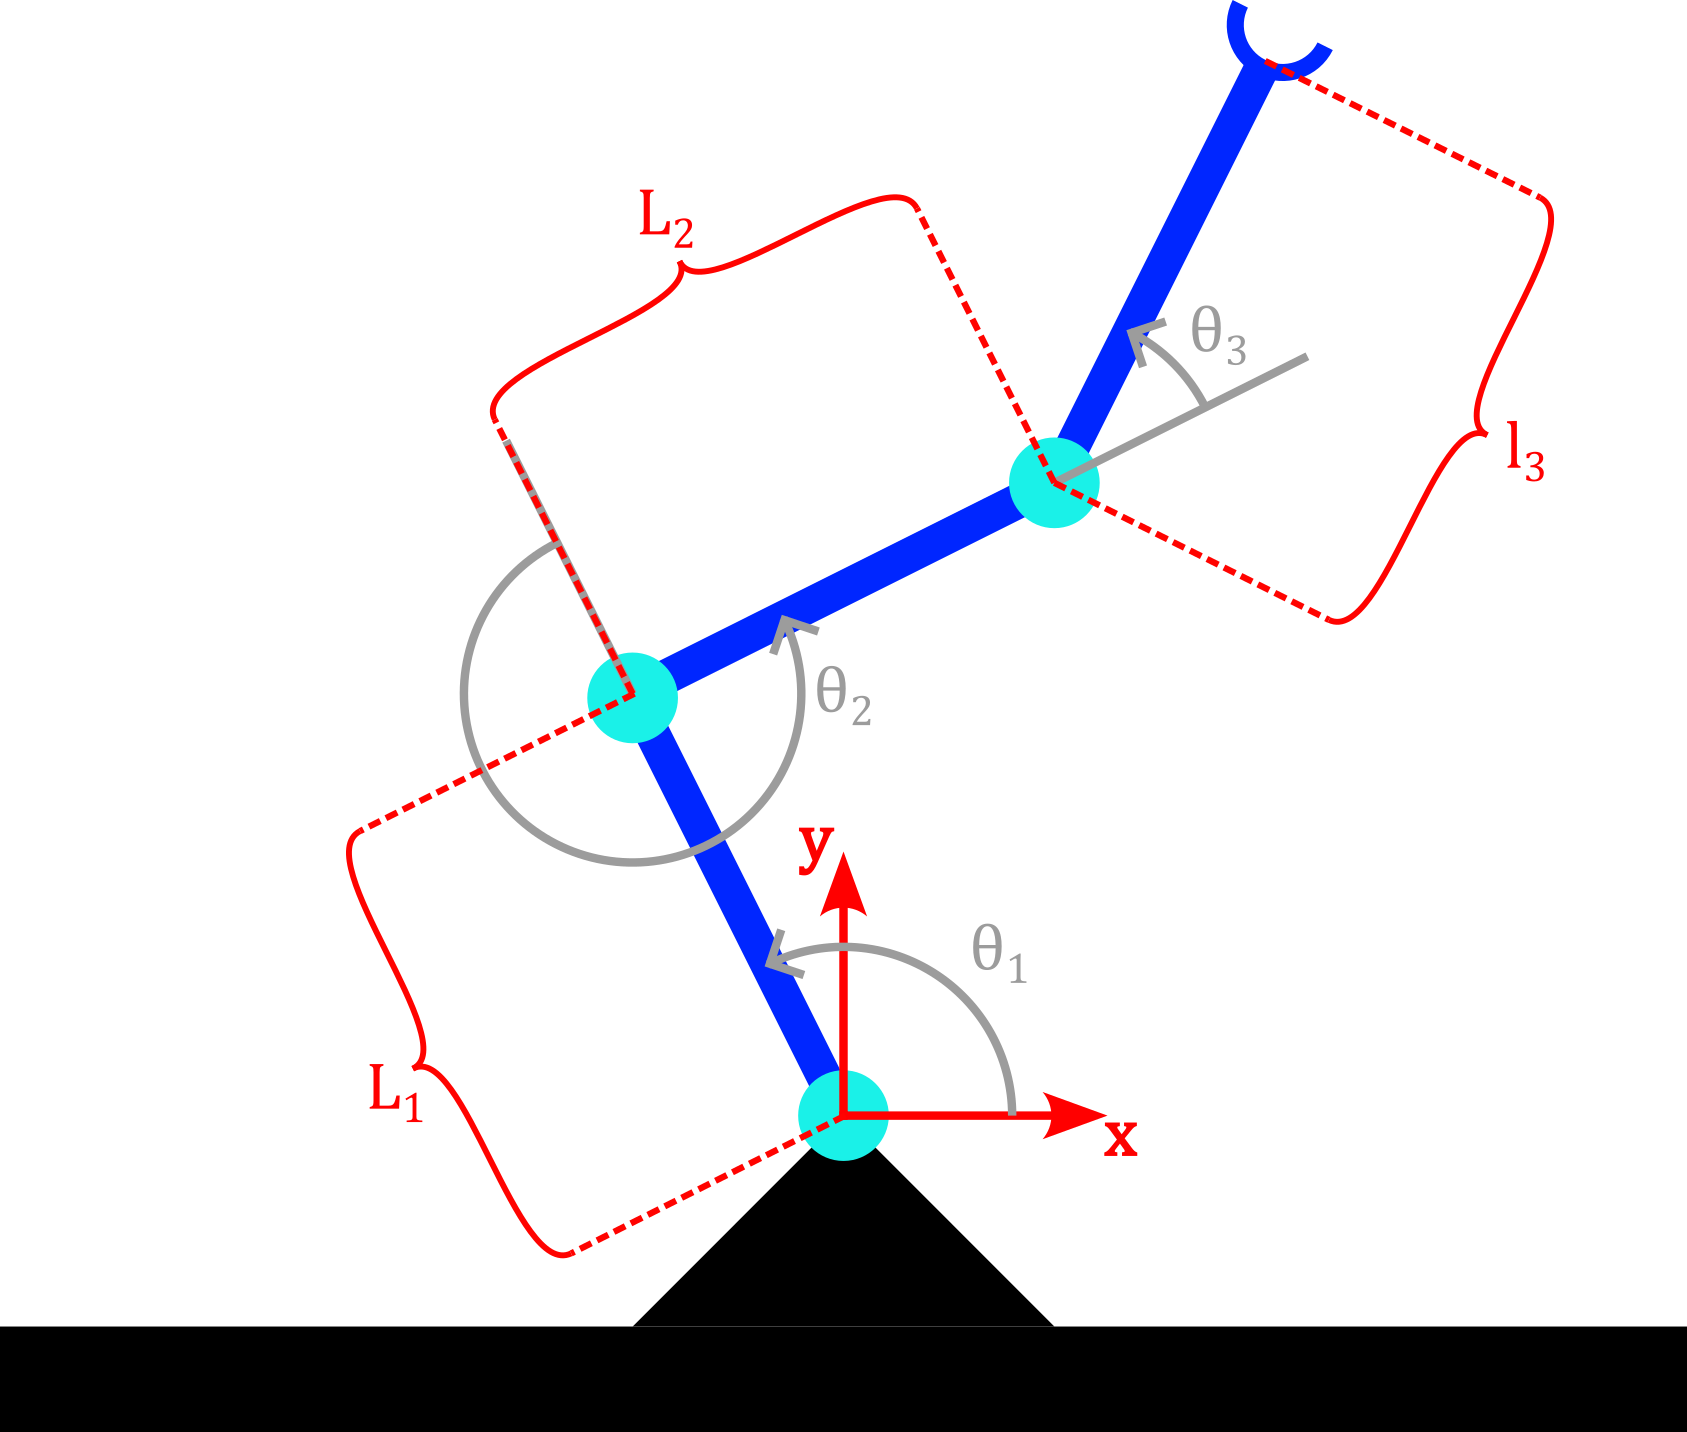
\includegraphics[width=0.5\textwidth]{Images/manipulator_inkscape.png}
    \caption{A 3-link planar robotic arm in $\mathbb{R}^2$.}
    \label{fig:robotic_link_arm}
\end{figure}

\subsubsection{Jacobian Matrix}

The Jacobian matrix relates small changes in joint angles to end-effector motion. As shown in equation \ref{eq:infinitesimal_change}, infinitesimal changes are described by partial derivatives \cite{modsim}. The Jacobian matrix $\bm{J}$ (equation \ref{eq:jacobian}) maps joint angle changes to end-effector position changes (equation \ref{eq:jacobian_pos_mapping}). Using the chain rule on equation \ref{eq:robot_kinematics} yields equation \ref{eq:jacobian_speed_mapping}, relating joint and end-effector velocities.

\begin{equation}
    \label{eq:infinitesimal_change}
    \delta  y = \frac{\partial y}{\partial x} \delta x
\end{equation}

\begin{equation}
    \label{eq:jacobian}
    \bm{J} = \begin{bmatrix}
        \frac{\partial x}{\partial q_1} & \frac{\partial x}{\partial q_2} & \cdots & \frac{\partial x}{\partial q_n} \\
        \frac{\partial y}{\partial q_1} & \frac{\partial y}{\partial q_2} & \cdots & \frac{\partial y}{\partial q_n}
    \end{bmatrix}
\end{equation}

\begin{equation}
    \label{eq:jacobian_pos_mapping}
    \bm{\delta x} = \bm{J}\bm{\delta q}
\end{equation}

\begin{equation}
    \label{eq:jacobian_speed_mapping}
    \bm{\dot x} = \bm{J}\bm{\dot q}
\end{equation}

    \subsubsection{Force/Torque Mapping}
    \label{sec:force_torque_mapping}

    For a robotic manipulator with $n$ joints (like figure \ref{fig:robotic_link_arm}), joint angles $q_i$ and torques $\tau_i$, the joint torques needed to support an end-effector force $F$ are given by equation \ref{eq:force_torque_mapping} \cite{ASADA_LECTURE_NOTES}.

    This relationship follows from the principle of virtual work. Consider virtual displacements $\delta q_i$ of joint angles and $\bm{\delta x}$ of end-effector position. Virtual displacements need only satisfy geometric constraints, not dynamic laws \cite{ASADA_LECTURE_NOTES}.

    For joint torques $\bm{\tau} = [\tau_1, \tau_2, ..., \tau_n]$ and end-effector force $\bm{-F}$, the virtual work is:

    \begin{equation}
        \label{eq:virtual_work}
        \bm{\delta W} = \bm{\tau^T\delta q -F^T\delta x} 
    \end{equation}
    At equilibrium, virtual work is zero for all valid displacements. Setting $\bm{\delta W} = 0$ and substituting $\bm{\delta x} = \bm{J}\bm{\delta q}$ from equation \ref{eq:jacobian_pos_mapping} gives:

    \begin{equation}
        \label{eq:force_torque_mapping}
        \bm{\tau} = \bm{J^T F}
    \end{equation}

    \subsubsection{Inverse Kinematics}
    Inverse kinematics calculates joint angles needed for a desired end-effector position. For a planar two-link manipulator with link lengths \(L_1\) and \(L_2\), we can solve analytically for joint angles \(\theta_1\) and \(\theta_2\) given target position \((x,y)\).

    The forward kinematics are described by the 2-link case of equation \ref{eq:robot_kinematics}.
    
    \begin{equation}
    x = L_1 \cos(\theta_1) + L_2 \cos(\theta_1 + \theta_2)
    \end{equation}
    
    \begin{equation}
    y = L_1 \sin(\theta_1) + L_2 \sin(\theta_1 + \theta_2)
    \end{equation}
    
    Using the law of cosines:
    
    \begin{equation}
    \theta_2 = \pm \arccos\left(\frac{x^2 + y^2 - L_1^2 - L_2^2}{2L_1L_2}\right)
    \end{equation}
    
    Then:
    
    \begin{equation}
    \theta_1 = \arctan2(y,x) - \arctan2(L_2\sin(\theta_2), L_1 + L_2\cos(\theta_2))
    \end{equation}
    
    The ± in \(\theta_2\) indicates two possible solutions exist for most positions - one with elbow up and one with elbow down. When \(L_1 = L_2\), the position \((0,0)\) is a singularity with infinite solutions. At the workspace boundary where \(x^2 + y^2 = (L_1 + L_2)^2\), only one solution exists.

\subsection{Contact Friction}
\label{sec:contact_friction}
Contact friction is a force that resists relative motion between surfaces. The classical Coulomb friction model \cite{modern_robotics_book} states that the friction force \(F_f\) is proportional to the normal force \(F_N\):

\begin{equation}
\label{eq:coulomb_friction}
F_f = \mu F_N
\end{equation}

where \(\mu\) is the coefficient of friction. This model distinguishes between static friction (surfaces at rest) and kinetic friction (surfaces in motion), with \(\mu_s > \mu_k\). The friction force opposes motion and is limited by:

\begin{equation}
\label{eq:friction_inequality}
|F_f| \leq \mu_s F_N \text{ (static)}
\end{equation}

When motion occurs, the friction force becomes:

\begin{equation}
\label{eq:kinetic_friction}
F_f = -\mu_k F_N \text{sign}(v)
\end{equation}

where \(v\) is the relative velocity. This discontinuity at \(v=0\) creates numerical challenges in simulation, often addressed by smoothing the transition between static and kinetic friction.

\subsection{Numerical Solvers}
\label{sec:numerical_solvers}

Contact dynamics simulation requires specialized numerical solvers due to discontinuities and rapid force changes during impacts. These dynamics need stiff solvers to accurately model the fast transitions in forces and velocities \cite{stiff_contact_ODE_1}\cite{stiff_contact_ODE_2}. Stiff solvers handle problems with widely varying timescales, maintaining stability during contact events. Standard solvers can become unstable or fail to converge. MATLAB's ode15s and ode23s are examples of stiff solvers designed for these challenging differential equations \cite{MATLAB_ODE}.


\subsection{Linear Least Squares Regression}
Linear least squares regression is a method for finding the best-fitting line through a set of points by minimizing the sum of squared residuals \cite{numerical_methods}. Given a set of observations \((x_i, y_i)\) and a linear model \(y = X\beta\), where \(X\) is the matrix of input variables and \(\beta\) contains the model parameters, the residual \(r_i\) for each observation is:

\begin{equation}
\label{eq:residual}
r_i = y_i - X_i\beta
\end{equation}

The sum of squared residuals \(S\) is then:

\begin{equation}
\label{eq:sum_squared_residuals} 
S = \sum_{i=1}^n r_i^2 = (y - X\beta)^T(y - X\beta)
\end{equation}

To minimize \(S\), we take its derivative with respect to \(\beta\) and set it to zero:

\begin{equation}
\label{eq:derivative_residuals}
\frac{\partial S}{\partial \beta} = -2X^T(y - X\beta) = 0
\end{equation}

Solving for \(\beta\) yields the normal equations:

\begin{equation}
\label{eq:normal_equations}
X^TX\beta = X^Ty
\end{equation}

The solution is therefore:

\begin{equation}
\label{eq:least_squares_solution}
\beta = (X^TX)^{-1}X^Ty
\end{equation}

This solution minimizes the sum of squared residuals and provides the optimal parameters \(\beta\) in the least squares sense.

\subsection{Mean Squared Error}
Mean Squared Error (MSE) measures the average squared difference between predicted values and actual values \cite{numerical_methods}. For a set of \(n\) predictions \(\hat{y}_i\) and corresponding true values \(y_i\), MSE is defined as:

\begin{equation}
\label{eq:mse}
\text{MSE} = \frac{1}{n}\sum_{i=1}^n (y_i - \hat{y}_i)^2
\end{equation}

MSE penalizes larger errors more heavily due to the squared term, making it useful for evaluating model fit quality. A lower MSE indicates better model performance.


\subsection{Moving Average Filter}
A moving average filter smooths data by replacing each point with the average of a window of neighboring points \cite{signal_processing}. For a window size \(w\), the filtered value \(y_i\) at index \(i\) is:

\begin{equation}
\label{eq:moving_average}
y_i = \frac{1}{w}\sum_{j=i-\lfloor w/2 \rfloor}^{i+\lfloor w/2 \rfloor} x_j
\end{equation}

where \(x_j\) are the input values. The filter reduces high-frequency noise while preserving lower-frequency trends in the data. Larger window sizes provide more smoothing but can attenuate rapid changes in the signal.

\subsection{Centered Finite Differences}
Centered finite differences approximate derivatives using symmetric sampling around each point \cite{numerical_methods}. For time series data with constant time step \(\Delta t\), the first and second derivatives at index \(i\) are approximated as:

\begin{equation}
\label{eq:first_derivative}
\dot{x}_i = \frac{x_{i+1} - x_{i-1}}{2\Delta t}
\end{equation}

\begin{equation}
\label{eq:second_derivative}
\ddot{x}_i = \frac{x_{i+1} - 2x_i + x_{i-1}}{(\Delta t)^2}
\end{equation}

\subsection{Inertia}
\label{sec:inertia}
The moment of inertia, \(I\), quantifies the rotational inertia of an object \cite{taylor_mechanics}, indicating how much torque is required for a desired angular acceleration.

\subsubsection{Parallel Axis Theorem}
The Parallel Axis Theorem \cite{taylor_mechanics} allows the calculation of the moment of inertia of a body about any axis, given its moment of inertia about a parallel axis through its center of mass. It is mathematically expressed as:

\begin{equation}
\label{eq:parallel_axis_theorem}
I = I_{\text{cm}} + md^2
\end{equation}

where:
\begin{itemize}
    \item \(I\) is the moment of inertia about the chosen axis,
    \item \(I_{\text{cm}}\) is the moment of inertia about the center of mass axis,
    \item \(m\) is the mass of the object,
    \item \(d\) is the distance between the two parallel axes.
\end{itemize}

\subsubsection{Thin Rod}
For a thin rod of length \(l\) and mass \(m\), rotating about an axis perpendicular to the rod and passing through its end, the moment of inertia is derived using the Parallel Axis Theorem. The moment of inertia about the center of mass is \cite{taylor_mechanics}:

\begin{equation}
\label{eq:rod_cm_inertia}
I_{\text{cm, rod}} = \frac{1}{12}ml^2
\end{equation}

Applying the Parallel Axis Theorem with \(d = \frac{l}{2}\):

\begin{equation}
\label{eq:rod_total_inertia}
I_{\text{rod}} = I_{\text{cm, rod}} + m\left(\frac{l}{2}\right)^2 = \frac{1}{12}ml^2 + \frac{1}{4}ml^2 = \frac{1}{3}ml^2
\end{equation}

\subsubsection{Disk}
For a solid disk of radius \(r\) and mass \(m\), the moment of inertia about its center is \cite{taylor_mechanics}:

\begin{equation}
\label{eq:disk_cm_inertia}
I_{\text{cm, disk}} = \frac{1}{2}mr^2
\end{equation}

Using the Parallel Axis Theorem to find the moment of inertia about an axis parallel and a distance \(d\) away:

\begin{equation}
\label{eq:disk_total_inertia}
I_{\text{disk}} = I_{\text{cm, disk}} + md^2 = \frac{1}{2}mr^2 + md^2
\end{equation}




